\section{Design}
\label{Design}
%section on all the design details
The specifications for this Sigma-Delta modulator to meet are shown in table \ref{tab:SDspec}.
These specifications are a relatively low signal bandwidth and a very high SNDR that is characteristic of an audio band ADC.
In this section different options are evaluated and chosen from to meet these specifications.

\begin{table}
    \begin{center}
    \caption{A summary of the specifications required for this Sigma-Delta ADC.}
    \label{tab:SDspec}
    \begin{tabular}{l l} 
        \toprule
        Specification   &   Value  \\
        \midrule
        Supply Voltage ($V_{dd}$)               & $3.3 V$              \\
        Differential Input Voltage              & $1.8 V_{rms}$        \\
        Reference voltage $V_{refn}$            & $ 0 V$               \\
        Refererence voltage $V_{refp}$          & $0.9 \times V_{dd}$  \\
        Signal to Noise Ratio                   & $103 dB$             \\
        Total Harmonic Distortion at full-scale & $-85 dB$             \\
        NO audio band limit cycles or tones     & N/A                  \\
        A flat audio band noise profile         & N/A                  \\
        Exclusive voltage references            & N/A                  \\
        Clock Frequency                         & $12.288 MHz$         \\
        \end{tabular}
    \end{center}
\end{table}


\subsection{Noise in  Switched Capacitor Integrators}
\label{Design:noise}
%estimating the capacitor sizes for different OSRs
%use this to compare designs
For any size of modulator the noise will be dominated by the first integrator at the input\cite{Henderson2013}.
Shown in table \ref{tab:capsizes} are the required input capacitor sizings for different OSRs and for a presumed SNDR of 106dB for a small margin on the specifications.
Also shown in table \ref{tab:capsizes} are the required $g_{m}$s of the amplifiers in the first integrator for these capacitor sizes and settling errors required.

Quantisation noise is intended to be a very small part of the noise budget(\cite{Steensgaard2004}, p.437) - making the initial SNDR target 123dB.
The capacitor sizes are found by equating the expected quantisation noise for a 123dB SNDR with the expected kT/C noise on the capacitor:
%example calculation
\begin{align}
    \frac{m k T}{C OSR} = N_{q}^{2} = \frac{V_{inRMS}^{2}}{10^{\frac{SNDR}{10}}} = \frac{1.8^{2}}{10^{\frac{106}{10}}} = 8.14\e{-11} \\
    C = \frac{m k T}{OSR N_{q}^{2}} = \frac{4 \times 1.23\e{-23} \times 293}{OSR \times 8.14\e{-11}} 
\end{align}
%explain symbols here
Where $V_{inRMS}$ is the RMS differential voltage range and $m=4$ for a differential circuit.

%assume linear settling for the g_m
To find the required g_{m}, linear settling is assumed, and the settling time is dependent on OSR:
\begin{align}
    \tau_{settling} = \frac{256\times T_{clk}}{2\times OSR}
\end{align}
Where $\tau_{settling}$ is the settling time.
To settle to within $\sqrt{8.14\e{-11}} = 9.02\e{-6} V_{RMS}$ over the $1.8 V_{RMS}$ range of the circuit:
\begin{align}
    e^{\frac{-\tau_{settling} g_{m}}{C}} = \frac{9.02\e{-6}}{1.8} \\
    g_{m}  = - \frac{C \times \ln{\frac{9.02\e{-6}}{1.8}}}{\tau_{settling}}
\end{align}

\begin{table}
    \begin{center}
    \caption{A table summarising the required capacitor sizes and amplifier $g_{m}$s for different OSRs.}
    \label{tab:capsizes}
    \begin{tabular}{l l p{0.3\textwidth}} 
    \toprule
    OSR & Required Capacitor Size (F) & Required Amplifier $g_{m}$ (S) \\ 
    \midrule
    2   &  8.855\e{-11}  & 2.305\e{-4}  \\
    4   &  4.427\e{-11}  & 2.305\e{-4}  \\
    8   &  2.214\e{-11}  & 2.305\e{-4}  \\
    16  &  1.107\e{-11}  & 2.305\e{-4}  \\
    32  &  5.534\e{-12}  & 2.305\e{-4}  \\
    64  &  2.767\e{-12}  & 2.305\e{-4}  \\
    128 &  1.384\e{-12}  & 2.305\e{-4}  \\
    256 &  6.918\e{-13}  & 2.305\e{-4}  \\
    \end{tabular}
    \end{center}
\end{table}


Neglecting second order effects it appears that there is no downside to choosing a high OSR in the design of a Sigma-Delta modulator.
Effects such as slew rate and switch delays will affect these problems, however.
Without more complex simulation analysis it is difficult to quantify these other effects and it can only be said that these effects will exist.
Therefore, a high OSR is recommended for this design.

\subsection{Modulator Choice}
%based on the different combinations of bits, order and OSR that could meet the required specification
Shown in table \ref{tab:modoptions} are the major possible options that are projected based on graphs by Schreier and Temes\cit{textbook} and lecture notes.
This list is also limited to the options that are possible using the provided tools.

%list all the optimised cifb designs
%and MASH options
%and silva-steensgard
%and multiple bit quantiser designs
\begin{table}
    \begin{center}
    \caption{A table summarising design options evaluated during the design.}
    \label{tab:modoptions}
    \begin{tabular}{l l l p{0.2\textwidth} p{0.2\textwidth}}
    \toprule
    Architecture  & Order &   OSR     & Peak Nominal Observed SNDR(dB) & Notes \\
    \midrule
    CIFB & 3     & 128 & 109.0 & Margin on specifications not high enough. \\
    CIFB & 3     & 256 & 128.1 & \\
    MASH & 2+1   & 128 & 126.8 & Stable, established design. \\
    MASH & 1+1+1 & 128 & 126.9 & Error correcting abilities less effective than 2+1 design. \\
    %Silva-Steensgaard & 2 &  does not meet spec without multi-bit feedback
    %multi-bits go here
    \end{tabular}
    \end{center}
\end{table}


This list is reduced in that many of the CIFB designs are impossible to realise due to time constraints - they would require learning how to edit Simulink designs to add different quantisers and additional modulator stages.
Initial attempts to edit Simulink designs were unsuccessful, therefore limiting the possibilities to third order designs with different OSRs.

%discussion of MASH converter designs
It was possible to use MASH converter designs existing to meet the specifications with a lower OSR than would be required by a CIFB design.
Unfortunately it has been shown in section \ref{Design:noise} that this is not a first order concern - in fact, it's recommended to pick the highest possible OSR.
A problem with MASH converter designs anticipated would be noise leakage(\cite{Schreier2004}, p.132) - due to mismatches in the transfer functions of the different stages.

An additional problem with a MASH converter design is that simulations showed it would not have a completely flat audio band noise profile.
This can be seen in figure \ref{fig:MASHnominal} and can be compared with figure \ref{fig:cifbnominal}.

\begin{figure}
    \begin{center}
    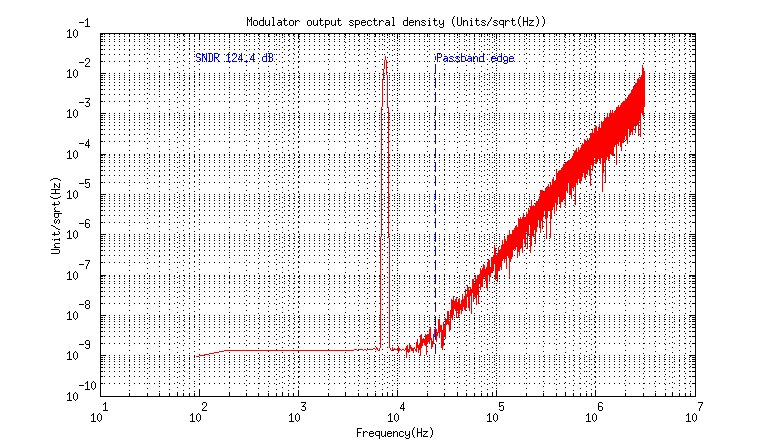
\includegraphics[width=0.8\textwidth]{MASHnominal.png}
    \label{fig:MASHnominal}
    \caption{An example of a possible nominal MASH SNDR profile with a sine wave input.}
    \end{center}
\end{figure}

\begin{figure}
    \begin{center}
    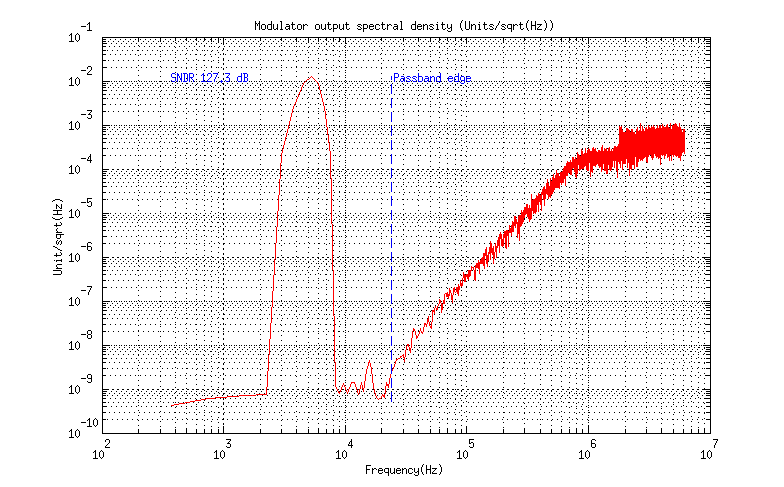
\includegraphics[width=0.8\textwidth]{cifbnominal.png}
    \label{fig:cifbnominal}
    \caption{An example of a possible nominal MASH SNDR profile with a sine wave input.}
    \end{center}
\end{figure}

%need an argument against multi-bit feedback
%read textbook for this

%state choice and the reasons for the choice
Originally, a 3rd order CIFB design with an OSR of 256 was chosen as the design as it was able to meet the flat audio band noise profile requirement thanks to its optimised NTF.
Other advantages include it's simplicity with single-bit feedback and the anticipation of efficiency with the optimised transfer function.
Unfortunately, this design proved impossible due to stability and requirements for modification in Simulink that were unsuccessful.

The second choice was a MASH 2+1 converter with an OSR of 128.
Problems outlined above have been considered in the verification of the design in section \ref{Verification}.

    \subsection{Schematic}
    \label{Design:schematic}
    %top level diagram and some schematics showing how the sub-blocks should be implemented
    The top level functional diagram of a two stage 2+1 MASH modulator is shown in figure \ref{fig:MASH}.
    This design comprises several standard blocks that can be further broken down into their circuit implementations.

    %top level schematic
    %screencap from matlab
    \begin{figure}
        \begin{center}
        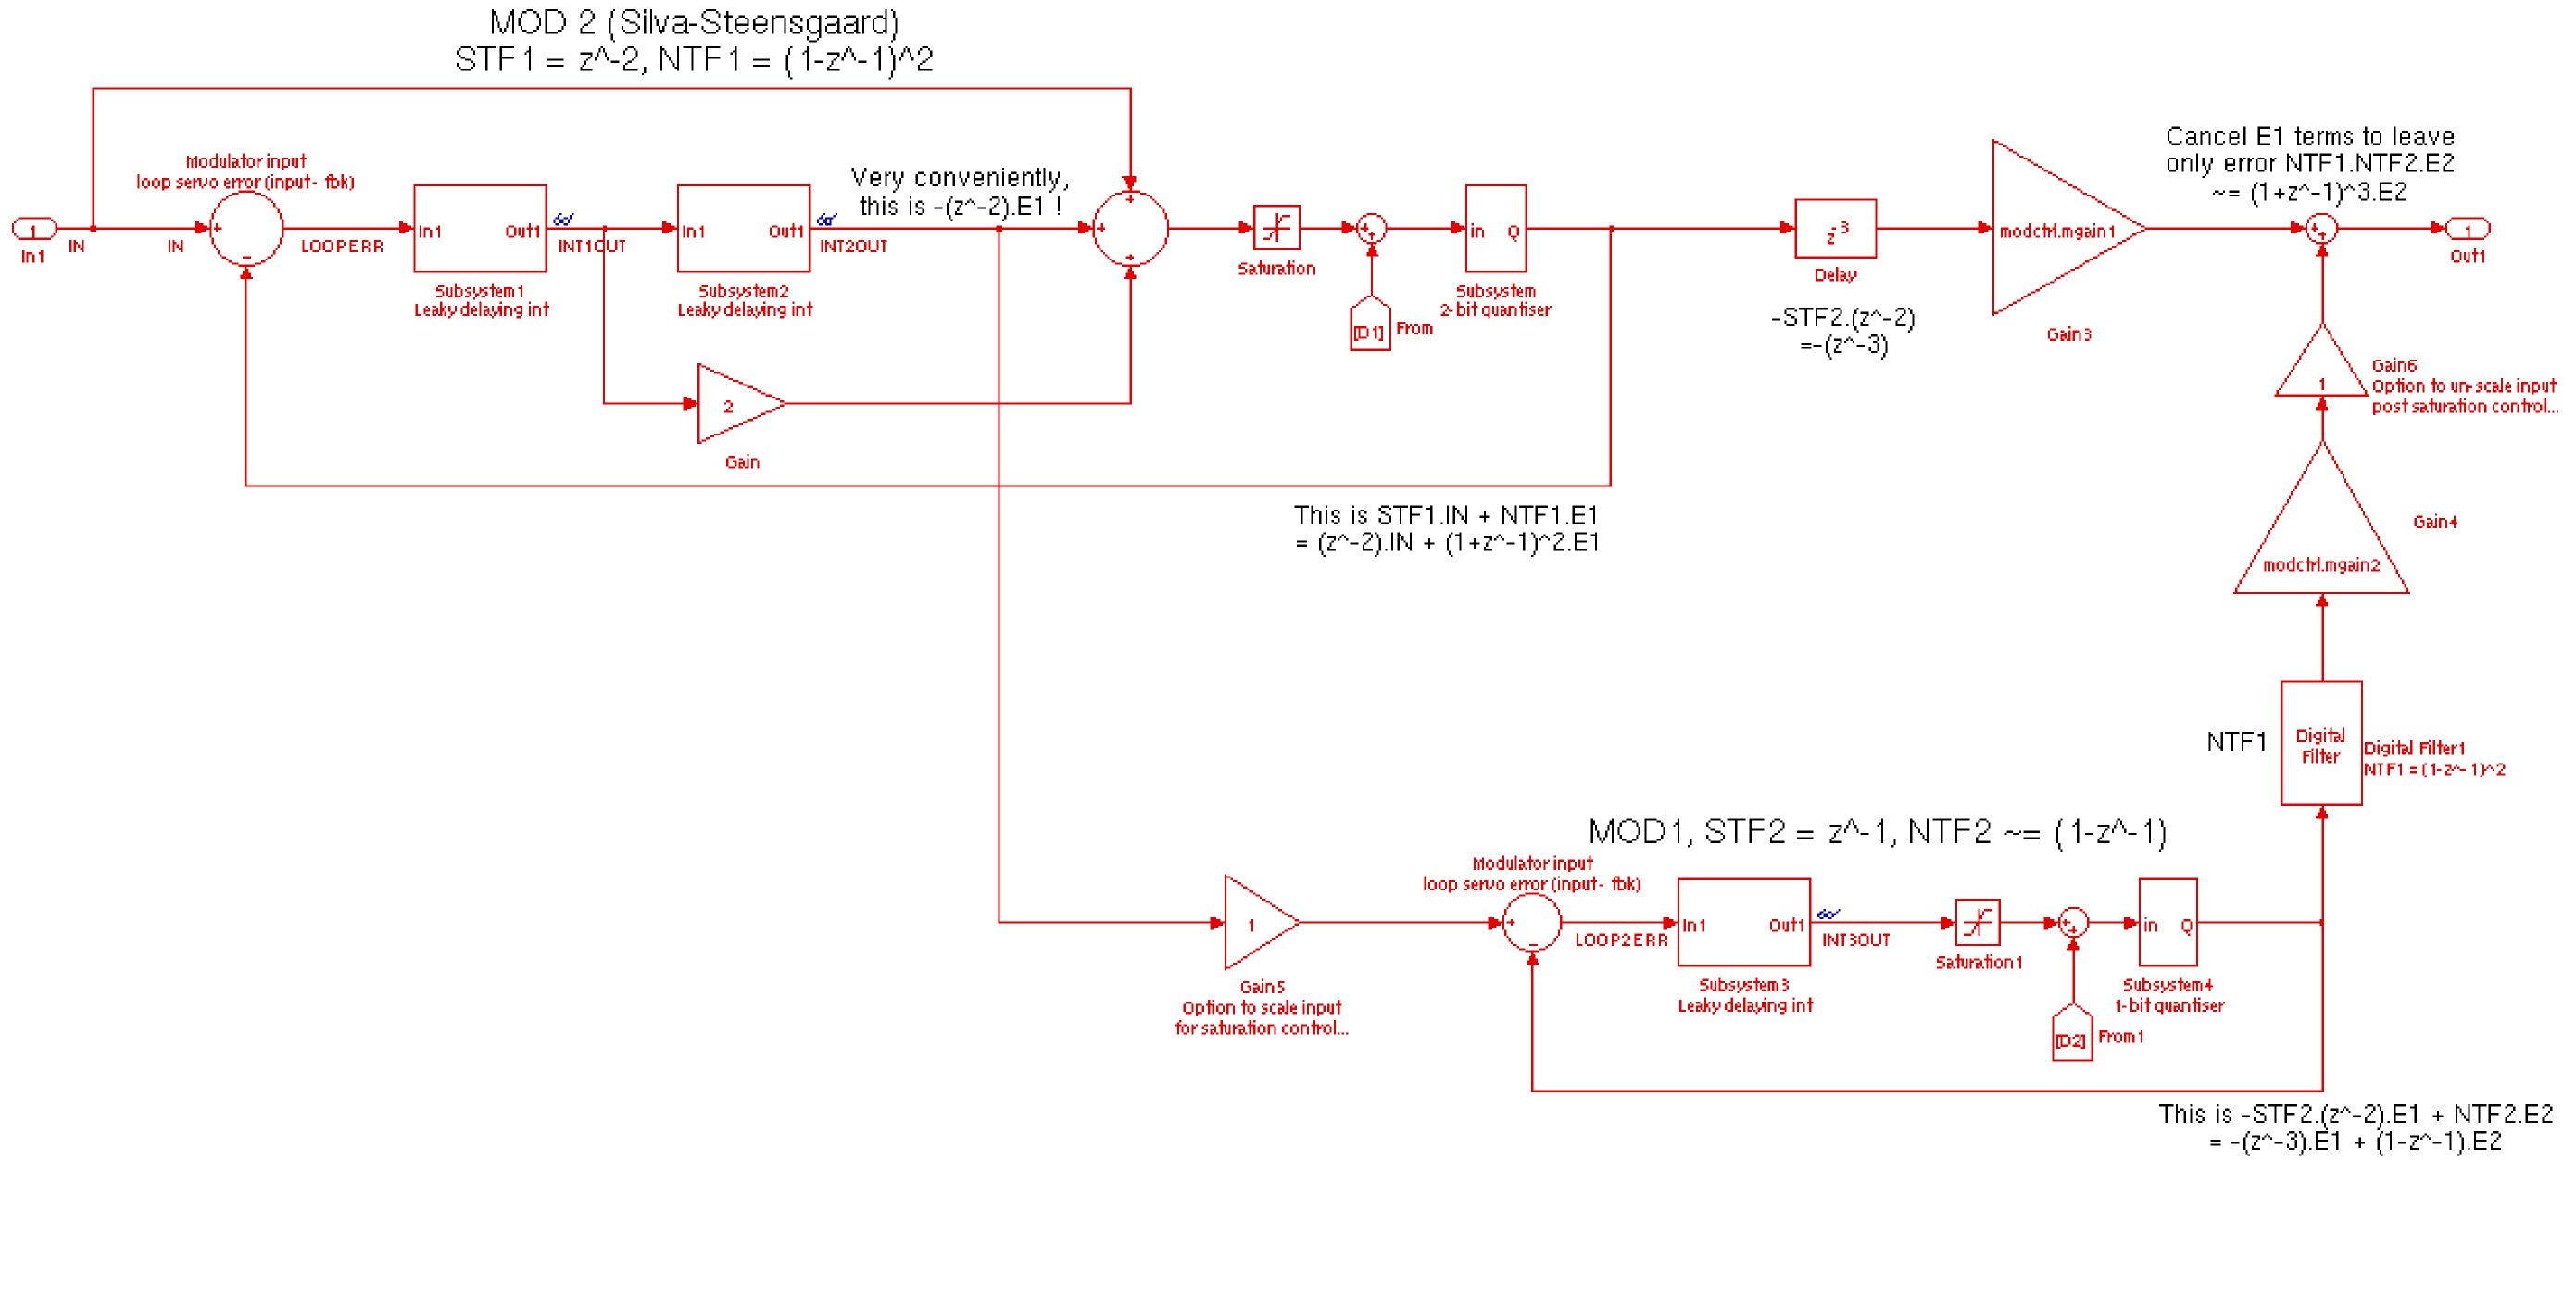
\includegraphics[height=0.8\textheight, angle=90]{MASH.png}
        \label{fig:MASH}
        \caption{Top level functional block diagram of the MASH modulator chosen in this design.}
        \end{center}
    \end{figure}

        \subsubsection{Silva-Steensgaard Modulator}
        %the second order modulator
        The first stage in this design is a second order modulator in a configuration known as a Silva-Steensgaard modulator.
        A differential circuit implementation of this circuit is shown in figure \ref{fig:silvaschematic}.

        \begin{figure}
            \begin{center}
            \includegraphics[height=0.8\textheight, angle=90]{silvaschematic.png}
            \label{fig:silvaschematic}
            \caption{A differential implementation on the Silva-Steensgaard modulator.}
            \end{center}
        \end{figure}

        %how to implement gain elements, coefficients, etc
        The gain elements and summing elements in this part of the design are implemented using capacitors.
        A differential multi-bit ADC and DAC must be implemented for this design to be created.
        A flash ADC implements the 2-bit ADC and an example circuit seen in figure \ref{fig:multiDAC} could be used to create the reference voltages if applied differentially.

        \begin{figure}
            \begin{center}
            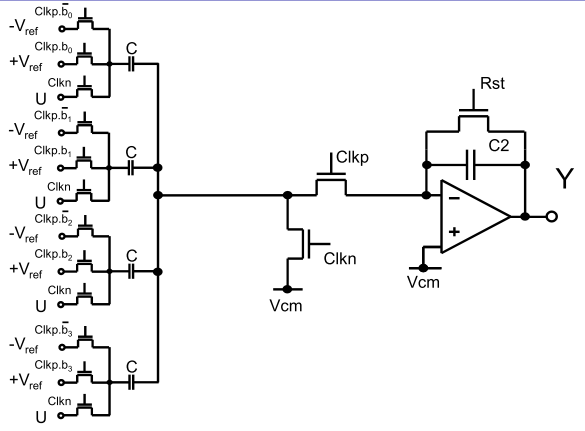
\includegraphics[width=0.8\textwidth]{multiDAC.png}
            \label{fig:multiDAC}
            \caption{A multi-bit DAC switched capacitor implementation\cite{Henderson2013a}.}
            \end{center}
        \end{figure}       

        %integrator design
        \subsubsection{First Order Modulator}
        %image and description of a differential integrator
        An example schematic for the first order modulator involved in this design is shown in figure \ref{fig:diffint}.
        This is the second modulator in the design and is a standard differential modulator design.

        %image should cite the lecture notes
        \begin{figure}
            \begin{center}
            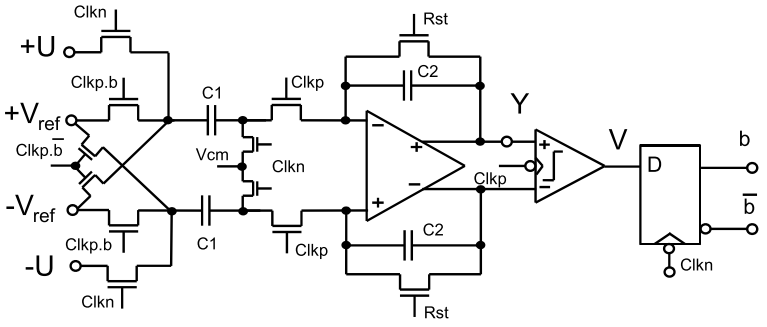
\includegraphics[width=0.8\textwidth]{diffint.png}
            \label{fig:diffint}
            \caption{A differential implementation of a first order modulator\cite{Henderson2013a}.}
            \end{center}
        \end{figure}

        %for the 1 bit quantiser
        A latched comparator is required to implement the single bit quantiser in the design.
        Designing this is a transistor level piece of design, and was not included in the design of the circuit.

        \subsubsection{Digital Signal Processing}
        %the filters, gain and digital summing elements
        The final signal processing in this modulator design is performed in the digital domain.
        A three cycle delay element, two gain operations and a summing element must be implemented in the digital design.
        This will also have to be combined with a digital filter after quantising prior to mixing.

        Without any of these components in the library available to the design at this point the implementation in Cadence could not be completed.
        It will be demonstrated that this design will be successful upon completion.

    \subsection{Component Sizing}
    \label{Design:components}
    %sizing of the capacitors and switches calculations
    The components in the first integrator are assumed to contribute the vast majority of the noise in the design.
    Due to this, only the switches and capacitors in this part of the design are considered in terms of their noise contribution.
    The required capacitor size for a 256 OSR and noise expectation comparable to an SQNR of 106dB is shown in table \ref{tab:capsizes}.

    The switches in the design must also be sized - similarly to the expected $g_{m}$ required for settling.
    Effective resistance of the switches must be designed in order that the voltage settles to within the required accuracy:   

    %take equation from above, then sub in R_on
    \begin{align}
        R_{switch}  = -\frac{\tau_{settling}}{C \ln{\frac{9.02\e{-6}}{1.8}}}
    \end{align}

    This evaluates to an effective switch resistance of $4819.59\Omega$.

    The required $g_{m}$ of the amplifier contributes to the required sizing of the input devices for the amplifier - along with estimations of bias currents required.
    An approximate minimum bias current can be estimated by the current required to slew the entire signal range in half a settling period.
    
    \begin{align}
        I = \frac{dV}{dt}C = \frac{2\times 1.8}{4.069\e{-8}}(6.918\e{-13}) = 6.121\e{-5} A
    \end{align}
    
    A bias current of approximately $100\mu A$ is therefore recommended in the input amplifier.
    Assuming an AMS process it is therefore possible to size the input devices for the settling requirements.
    
    \begin{align}
        g_{m} = \sqrt{\frac{2K'_{p} W |I_{D}|}{L}} \\
        \frac{W}{L} = \frac{g_{m}^{2}}{2K'_{p} |I_{D}|} = \frac{(2.305\e{-4})^{2}}{2(14\e{-6})(100\e{-6})} = 18.975
    \end{align}
    Where $K'_{p} = 14\mu A/V^{2}$ - assuming PMOS input devices for lower noise performance.
    Requirements for wider devices due to slewing or gain requirements could change this estimation, but it provides a lower bound.

    %remaining components, by estimating the noise factor of the amplifier
    The remaining components - switches and capacitors in the design - will all be sized smaller than those at the input as the input referred effect of these components will be negligible.
    Schreier \& Temes estimate the influence of capacitors in further stages to be approximately 0.01\%(\cite{Steensgaard2004}, p.441) of the input capacitor's contribution.
    From this, it can be estimated that capacitors of 20fF would be a safe value, and this would ease settling requirements in the circuit - switches could be up to 50 times more resistive, and therefore 50 times less wide.

\subsection{Conclusion}
\label{Design:conclusion}
%conclusion, write this at the end
The design of this circuit was mainly a process of choosing a modulator architecture and OSR.
Initial choices failed in simulation, forcing the choice of a dependable architecture.
A 2+1 MASH converter with an OSR of 128 was chosen and the sizes of the various components were estimated.

